\documentclass[pdf,11pt]{beamer}

\usepackage[utf8]{inputenc}
\usepackage{graphicx}       % Images
\graphicspath{{Images/}}
\usepackage{xcolor}         % Change Colors
\usepackage{caption}
\captionsetup[figure]{font=small}
\usepackage{multimedia}     % Movies!
\usepackage{tikz}           % Vectored pictures
%\usepackage{media9}
%\hypersetup{pdfpagemode=FullScreen} % Presentation Mode
\usepackage{animate}        % gifs
\usepackage{tikz}
\usepackage{amsmath}
\usepackage{amssymb}
\tikzset{
    ->,
    level distance = 12em,
    minimum size=2em,
    %edge from parent/.style={draw,thick},
    level 1/.style={sibling distance=6em},
    level 2/.style={sibling distance=3em},
    thick/.style = {line width=1.5pt},
    extra thick/.style = {line width=3.5pt},
    red node/.style={shape=circle,draw=red,fill=red!40,thick,inner sep=1.2},
    blue node/.style={shape=circle,draw=blue,fill=blue!40,thick,inner sep=1.2}
}

\tikzstyle{round}=[thick,draw=black,circle]

% Remove navigation symbols
\beamertemplatenavigationsymbolsempty
% Add page number
\addtobeamertemplate{navigation symbols}{}{%
    \usebeamerfont{footline}%
    \usebeamercolor[fg]{footline}%
    \hspace{1em}%
    \insertframenumber/\inserttotalframenumber
}

% Title
\title{UO 510: Normalizing Flow Research Project
}
\author{Luis Guzman \& Steven Walton\\ \small University of Oregon}
\date{3 June 2020}

\usebackgroundtemplate
{
    
\includegraphics[width=\paperwidth,height=\paperheight]{UO_Simple.png}
}
\definecolor{UOYellow}{HTML}{FDCB00}
\definecolor{UOGreen}{HTML}{424443}
%\newcommand{\mytitle}[1]{\setcolor{bg=UOYellow,fg=green}\frametitle{{#1}}}

% Formatting
%\setbeamercolor{title}{fg=white}
%\setbeamercolor{normal text}{fg=white}
%\setbeamercolor{structure}{fg=white}        % Adjusts figures and frame titles
%\setbeamertemplate{frametitle}[default][center]
%\setbeamerfont{frametitle}{size=\Huge}
%%\setbeamerfont{normal text}{size=\LARGE}
%%\setbeamerfont{structure}{size=\LARGE}
%\setbeamercolor{footline}{fg=UOGreen}
%%\setbeamerfont{footline}{series=\bfseries}


\begin{document}
\frame{\titlepage}

%%%%%%%%%%%%%%%%%%%%%%%%%%%%%%
% Use include for new sections
%%%%%%%%%%%%%%%%%%%%%%%%%%%%%%

\begin{frame}
\begin{itemize}
    \item \textbf{\color{red}{What are Normalizing Flows}}
    \item NICE
    \item RealNVP
    \item GLOW
    \item GamePlan
    \item Results
\end{itemize}
\end{frame}

\begin{frame}
\begin{itemize}
    \item What are Normalizing Flows
    \item \textbf{\color{red}{NICE}}
    \item RealNVP
    \item GLOW
    \item GamePlan
    \item Results
\end{itemize}
\end{frame}

\begin{frame}{NICE: Non-linear Independent Components Estimation}
\begin{itemize}
    \item Key contribution is finding a function with:
    \begin{itemize}
        \item Easy determinant
        \item Easy inverse
    \end{itemize}
    \item General coupling layer
    \begin{itemize}
        \item Create a partition of $x \in \mathbb{R}^D$ using $I_1 = [1, d]$ and $I_2 = [d, D]$
        \item Define $y = (y_{I_1}, y_{I_2})$
            \begin{align*}
                y_{I_1} &= x_{I_1} \\
                y_{I_2} &= g(x_{I_2}; m(x_{I_1}))
            \end{align*}
        \item $m : \mathcal{R}^d \longrightarrow \mathcal{R}^{D-d}$
        \item The Jacobian is $\frac{\partial y}{\partial x} =$
        $\begin{bmatrix}
            I_1 & 0 \\
            \frac{\partial y_{I_2}}{\partial x_{I_1}} &  \frac{\partial y_{I_2}}{\partial x_{I_2}}
        \end{bmatrix} = \frac{\partial y_{I_2}}{\partial x_{I_2}}$ 
    \end{itemize}
\end{itemize}
\end{frame}
\begin{frame}{NICE: Additive coupling layer}
\begin{itemize}
    \item Additive coupling law: $g(a; b) = a + b$
    \begin{align*}
                y_{I_1} &= x_{I_1} \\
                y_{I_2} &= x_{I_2} + m(x_{I_1})
    \end{align*}
    \item Inverse
    \begin{align*}
                x_{I_1} &= y_{I_1} \\
                x_{I_2} &= y_{I_2} - m(x_{I_1})
    \end{align*}
    \item Jacobian determinant
    \begin{align*}
        \text{det} = \frac{\partial y_{I_2}}{\partial x_{I_2}} = 1
    \end{align*}
    \item $m$ coupling functions are NN with linear outputs.
\end{itemize}
\end{frame}
\begin{frame}{NICE: layered architecture and scaling}
    \begin{itemize}
        \item Composing several layers
        \begin{itemize}
            \item More complex transformations
        \end{itemize}
        \item Part of the input unchanged
        \begin{itemize}
            \item Exchange the role of the two subsets
        \end{itemize}
        \item Volume preserving determinants
        \begin{itemize}
            \item Diagonal scaling matrix $S$ at the top layer.
        \end{itemize}
    \end{itemize}
\end{frame}
\begin{frame}{NICE: layered architecture and scaling}
\begin{align*}
    h_{I_1}^{(1)} &= x_{I_1}\\
    h_{I_2}^{(1)} &= x_{I_2} + m^{(1)}(x_{I_1})\\ 
    h_{I_2}^{(2)} &= h_{I_2}^{(1)}\\
    h_{I_1}^{(2)} &= h_{I_1}^{(1)} + m^{(2)}(x_{I_2})\\ 
    h_{I_1}^{(3)} &= h_{I_1}^{(2)}\\
    h_{I_2}^{(3)} &= h_{I_2}^{(2)} + m^{(3)}(x_{I_1})\\ 
    h_{I_2}^{(4)} &= h_{I_2}^{(3)}\\
    h_{I_1}^{(4)} &= h_{I_1}^{(3)} + m^{(4)}(x_{I_2})\\ 
    h &= \text{exp}(S) \odot h^{(4)}
\end{align*}
\end{frame}

\begin{frame}
\begin{itemize}
    \item What are Normalizing Flows
    \item NICE
    \item \textbf{\color{red}{RealNVP}}
    \item GLOW
    \item GamePlan
    \item Results
\end{itemize}
\end{frame}

\begin{frame}
    \frametitle{RealNVP (Luis)}
\end{frame}

\begin{frame}
\frametitle{GLOW}
    \begin{itemize}
        \item Flow-based generative model   
        \item Uses invertible 1x1 convolutions 
        \item Builds off of NICE and RealNVP (will leave out redundant info)
        \item Paper has a good overview of generative models and the
        differences.
    \end{itemize}
\end{frame}

\begin{frame}
\frametitle{Model}
\center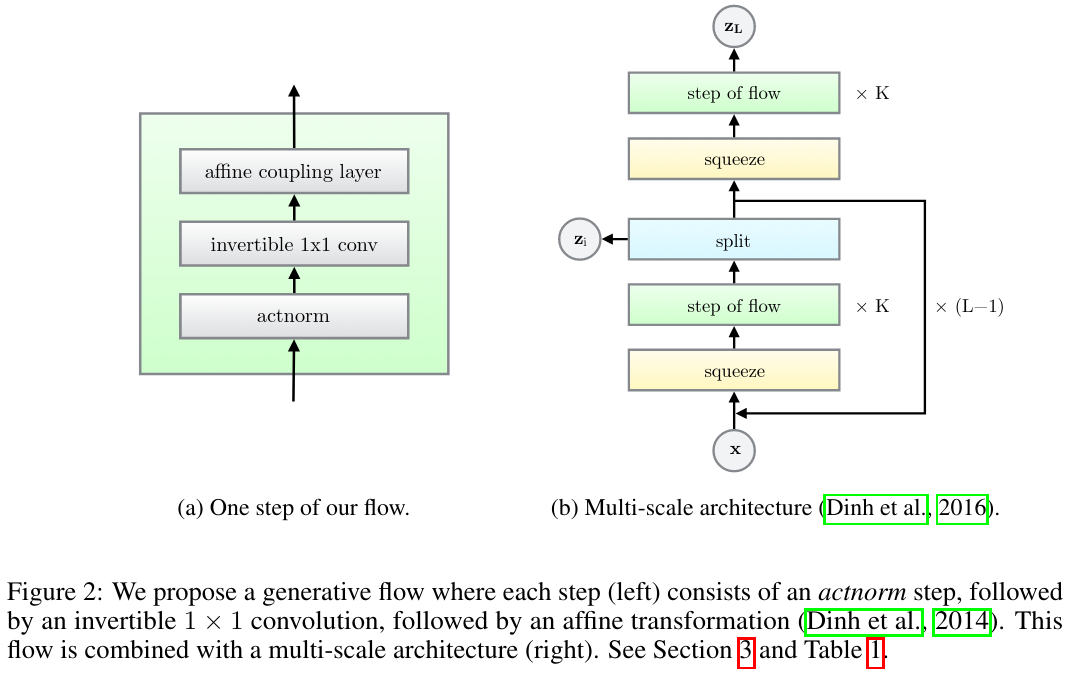
\includegraphics[width=0.8\textwidth]{GLOWModel.png}
\end{frame}

\begin{frame}
\frametitle{Model Components}
\center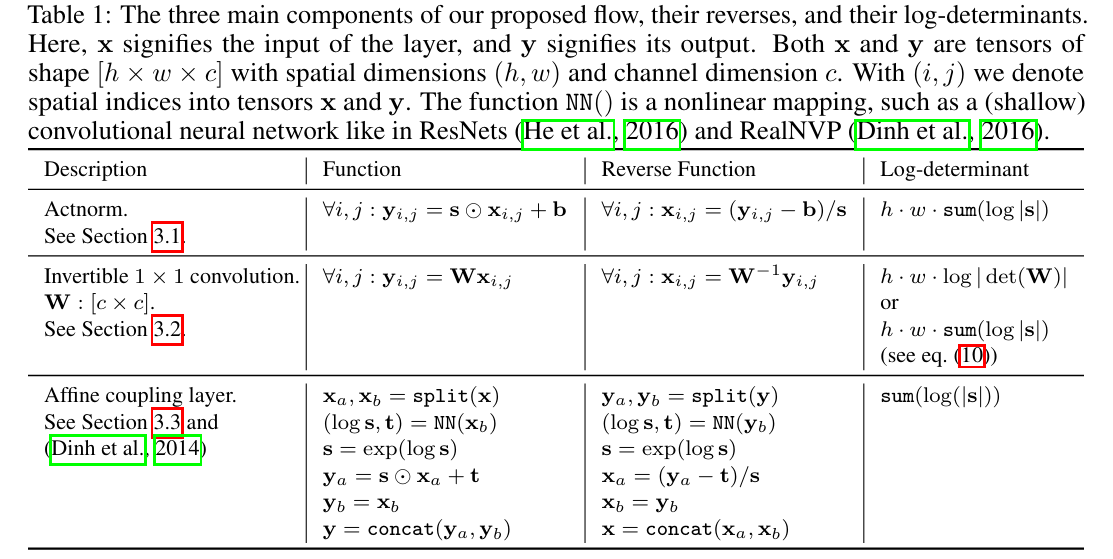
\includegraphics[width=0.8\textwidth]{GLOWComponents.png}
\end{frame}

\begin{frame}
\frametitle{Invertible 1x1 Convolutions}
    \begin{itemize}
        \item NICE uses a flow that uses a reverse permutation for channel ordering.
        \item GLOW learns this permutation with a 1x1 convolution
    \end{itemize}
    \begin{equation}
        log \left| det \left(\frac{d \textrm{conv2D}(\mathbf{h};\mathbf{W})}
                {d\mathbf{h}}\right)\right| = h \cdot w \cdot \log|det(\mathbf{W})| 
    \end{equation}
    \begin{itemize}
        \item Computing $\mathbf{W}$ can be reduced from $O(c^3)$ to $O(c)$ by
        LU Decomposition
    \end{itemize}
    \begin{align*}
        \mathbf{W} &= \mathbf{PL}(\mathbf{U} + diag(\mathbf{s}))\\
        log|det(\mathbf{W})| &= \sum(\log|\mathbf{s}|)
    \end{align*}
\end{frame}

\begin{frame}
\frametitle{Properties}
    \begin{itemize}
        \item Additive coupling layer has $\mathbf{s}=1$ and log-determinant = 0
        \item Zero initialization helps because they act like an identity
        \item Split and concatenation along channel dimension.
        \item Learned Permutation
    \end{itemize}
\end{frame}

\begin{frame}
\frametitle{GLOW Results}
\center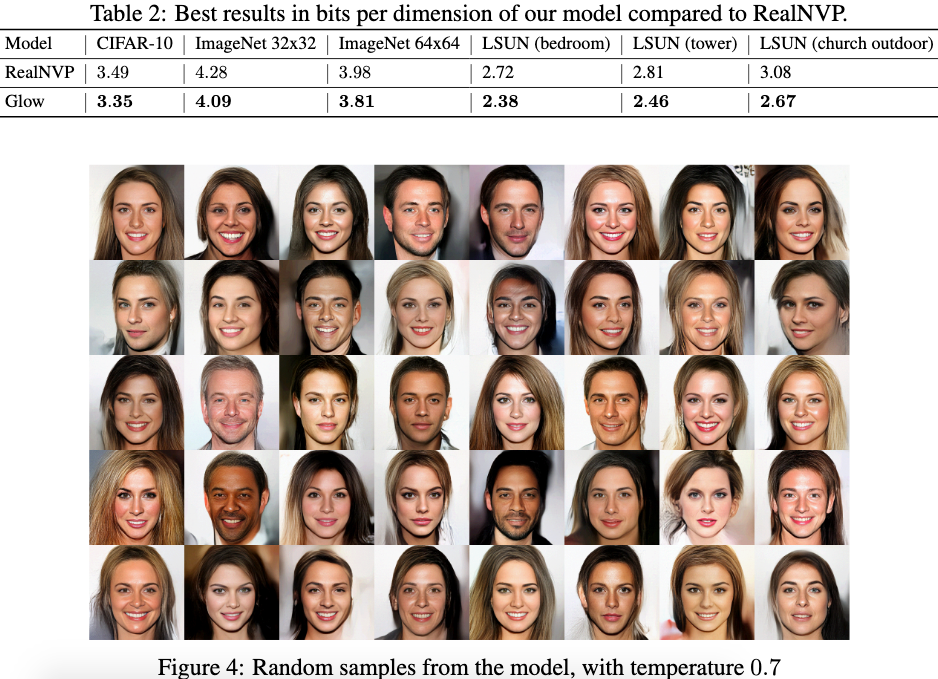
\includegraphics[width=0.8\textwidth]{GLOWResults.png}
\end{frame}

\begin{frame}
\begin{itemize}
    \item What are Normalizing Flows
    \item NICE
    \item RealNVP
    \item GLOW
    \item \textbf{\color{red}{GamePlan}}
    \item Results
\end{itemize}
\end{frame}

\begin{frame}
    \frametitle{GamePlan (Steven)}
    \begin{itemize}
        \item Read NICE, RealNVP, GLOW, FFJORD
        \item Independently replicate NICE and experiment with MNIST
        \item Upgrade to GLOW
        \item Retrain a common classifier to work on Kaggle Pneumonia dataset
        \item Adjust GLOW model to work on Pneumonia dataset
    \end{itemize}
\end{frame}

\section{Results}
In this section incrementally presents the results we obtained while working on the current project.
\subsection{NICE results}
As mentioned previously, we first implemented the NICE~\cite{nice} model. Figure~\ref{fig:forward_pass} showcases the the transformation of an input image after it has passed through the model. Given that NF models are completely reversible, if the transformed image shown in Figure~\ref{fig:transformed} is put through the backward pass of the model the original image (Figure \ref{fig:original}) is obtained.  Conversely, Figure \ref{fig:backward_pass} shows how images are generated by sampling a random vector from the prior distribution (multi-variate Gaussian in our experiments) and putting it through the backward pass of the NF model.
    \begin{figure}[htbp!]
     \centering
     \begin{subfigure}[b]{0.45\textwidth}
         \centering
         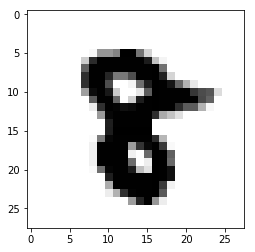
\includegraphics[width=0.5\textwidth]{input.png}
         \caption{Input image}
         \label{fig:original}
     \end{subfigure} 
     \hfill
     \begin{subfigure}[b]{0.45\textwidth}
         \centering
         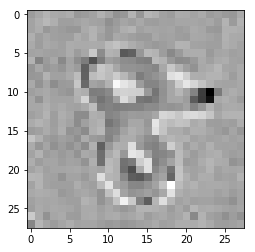
\includegraphics[width=0.5\textwidth]{transformed.png}
         \caption{Transformed}
         \label{fig:transformed}
     \end{subfigure}
     \hfill
     \caption{Transformation of an input image via forward pass.}
     \label{fig:forward_pass}
\end{figure}

    \begin{figure}[htbp!]
     \centering
     \begin{subfigure}[b]{0.45\textwidth}
         \centering
         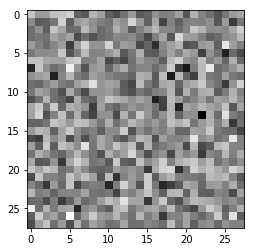
\includegraphics[width=0.5\textwidth]{sample.png}
         \caption{Sample from prior}
     \end{subfigure} 
     \hfill
     \begin{subfigure}[b]{0.45\textwidth}
         \centering
         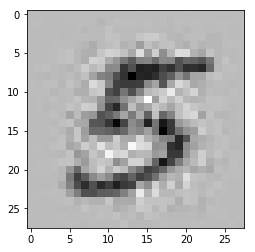
\includegraphics[width=0.5\textwidth]{generated.png}
         \caption{Generated image}
     \end{subfigure}
     \hfill
     \caption{Image generation with backward pass}
     \label{fig:backward_pass}
\end{figure}

The generation results after training two equivalent NICE models on both the MNIST and FashionMNIST data sets are shown in Figure~\ref{fig:nice_results}. The top image (\ref{fig:random_samples}) shows the vectors randomly sampled from the prior distribution, while the middle (\ref{fig:mnist_results}) and bottom (\ref{fig:fashion_results}) show the generated images created by transforming such sampled vectors by the MNIST and FashionMNIST models, respectively.

\begin{figure}[htbp!]
     \centering
     \begin{subfigure}[b]{0.3\textwidth}
         \centering
         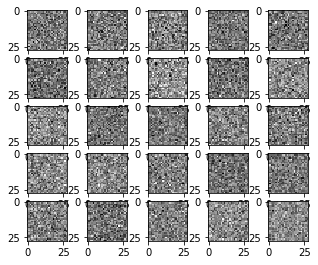
\includegraphics[width=\textwidth]{prior2.png}
         \caption{Sampled vectors}
         \label{fig:random_samples}
     \end{subfigure} 
     \hfill
     \begin{subfigure}[b]{0.3\textwidth}
         \centering
         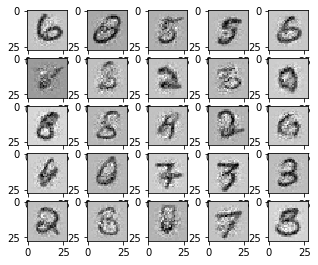
\includegraphics[width=\textwidth]{mnist2.png}
         \caption{MNIST}
         \label{fig:mnist_results}
     \end{subfigure}
     \hfill
     \begin{subfigure}[b]{0.3\textwidth}
         \centering
         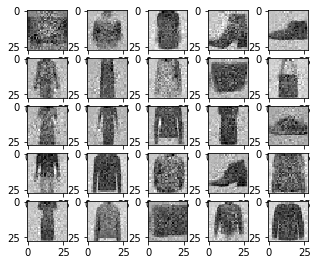
\includegraphics[width=\textwidth]{fashion2.png}
         \caption{FashionMNIST}
         \label{fig:fashion_results}
     \end{subfigure}
     \caption{NICE image generation results.}
     \label{fig:nice_results}
\end{figure}

It is apparent that the images generated by the NICE models are not great. We attribute this to the fact that the NICE normalizing flow is a very shallow one (using only 4 stacked layers), it only uses additive coupling layers, and relies on manually reversing the roles of the features partition subsets to ensure that all dimensions are transformed. All of these characteristics limit the models ability to learn complex distributions. 

\subsection{GLOW results}

Next we implemented the GLOW~\cite{glow} model. We purposely skipped implementing RealNVP~\cite{realnvp} because all of its innovations with respect to NICE, specifically the use of Affine coupling layers and the Multi-scale framework, are also used in GLOW. We trained our GLOW implementation on both CIFAR10 and the CelebA data sets. Here we present some results from the later one, which we find to be more relevant.

Figure~\ref{fig:glow_results} shows some image generation results for vectors sampled at different temperatures $\tau$. The images at the top row are sampled at $\tau = 0$ and thus all of the generated images are the same. The images at the bottom row are sampled at $\tau = 1$. It can be observed that as $\tau$ increases the presence of artifacts becomes more prevalent in the generated images. We found, empirically, that a $\tau$ value between $[0.2-0.6]$ yielded the best results, qualitatively.
    \begin{figure}
        \centering
        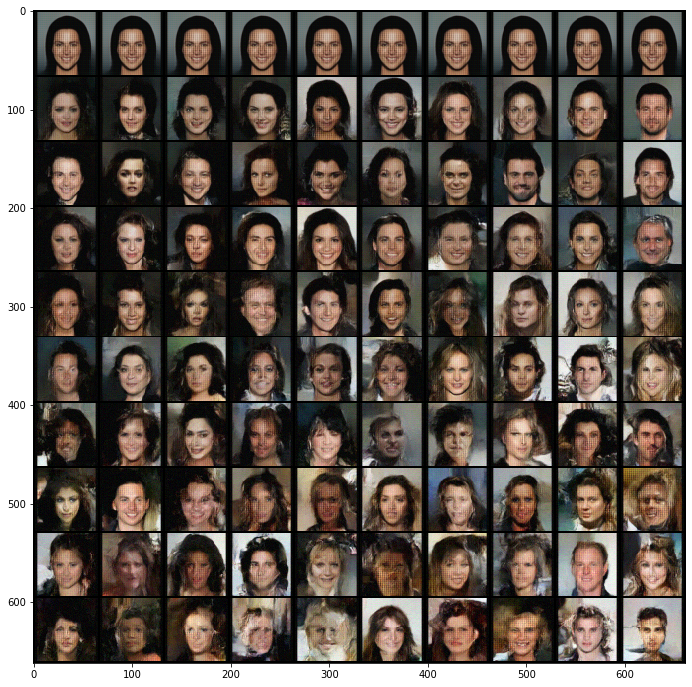
\includegraphics[width=0.5\textwidth]{celeb_multiple_stds2.png}
        \caption{GLOW generation results}
        \label{fig:glow_results}
    \end{figure}

We trained 2 distinct GLOW models with images with dimensionality of 64, and 128, respectively. Figure \ref{fig:glow_results2} shows some examples of the images generated by our models. While these results still do not achieve the same level of quality than the ones presented it the GLOW paper, we think they are sufficiently good given the computing resources available to us at the time. In particular, we were unable to train models that were as deep as the ones used in the original paper and also we could not train at 512 x 512 dimensionality.    

    \begin{figure}[htbp!]
     \centering
     \begin{subfigure}[b]{0.3\textwidth}
         \centering
         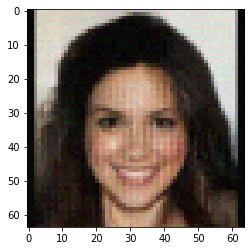
\includegraphics[width=\textwidth]{celeb_sample2.png}
         %\caption{MNIST}
     \end{subfigure}
     \hfill
     \begin{subfigure}[b]{0.3\textwidth}
         \centering
         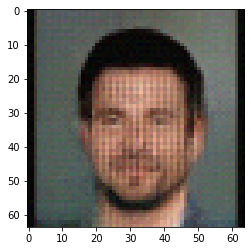
\includegraphics[width=\textwidth]{celeb_sample3.png}
         \caption{64 x 64 images}
     \end{subfigure}
     \hfill
     \begin{subfigure}[b]{0.3\textwidth}
         \centering
         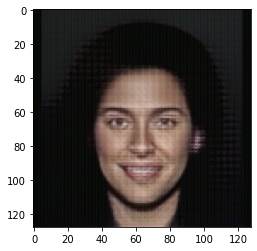
\includegraphics[width=\textwidth]{celeb_sample5.png}
         %\caption{MNIST}
     \end{subfigure}
     \hfill
     \begin{subfigure}[b]{0.3\textwidth}
         \centering
         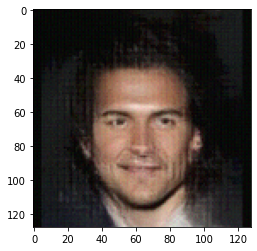
\includegraphics[width=\textwidth]{celeb_sample6.png}
         \caption{128 x 128 images}
     \end{subfigure}
     \hfill

     \caption{Images generated with GLOW}
     \label{fig:glow_results2}
\end{figure}

\subsection{X-ray data}

As discussed previously, our ultimate goal is to train a NF model that is able to fool a classifier. Thus, we first trained three distinct CNN-based (VGG19, Alexnet, Resnet50) classifiers on the Chest X-ray data set \footnote{https://www.kaggle.com/paultimothymooney/chest-xray-pneumonia}. Figure~\ref{fig:x_rays} shows some examples from both normal (\ref{fig:normal}) and pneumonia (\ref{fig:pneumonia}) images. Figure \ref{fig:classifiers_performance} shows the accuracy on the validation set for each of the classifiers. It can be observed that all of them achieve a fairly high validation accuracy of $\sim 90\%$.
    \begin{figure}
        \centering
        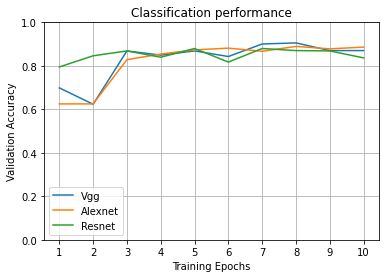
\includegraphics[width=.5\textwidth]{classification_performance.png}
        \caption{Classifiers validation performance.}
        \label{fig:classifiers_performance}
    \end{figure}
\begin{figure}[htbp!]
     \centering
     \begin{subfigure}[b]{0.3\textwidth}
         \centering
         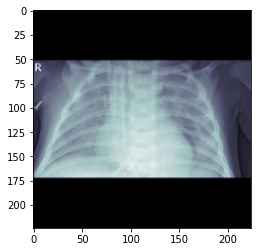
\includegraphics[width=\textwidth]{xray_normal1.png}
         %\caption{Sampled vectors}
     \end{subfigure} 
     \hfill
     \begin{subfigure}[b]{0.3\textwidth}
         \centering
         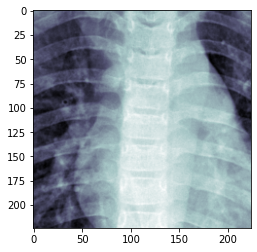
\includegraphics[width=\textwidth]{xray_normal3.png}
         \caption{Normal examples.}
         \label{fig:normal}
     \end{subfigure}
     \hfill
     \begin{subfigure}[b]{0.3\textwidth}
         \centering
         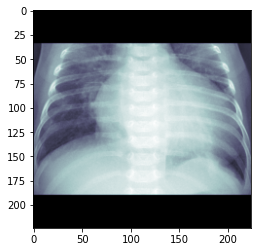
\includegraphics[width=\textwidth]{xray_pneumonia1.png}
         %\caption{Sampled vectors}
     \end{subfigure} 
     \hfill
     \begin{subfigure}[b]{0.3\textwidth}
         \centering
         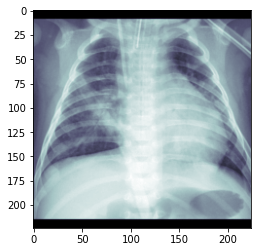
\includegraphics[width=\textwidth]{xray_pneumonia2.png}
         \caption{Pneumonia examples}
         \label{fig:pneumonia}
     \end{subfigure}
     \hfill
     \caption{Samples from X-ray dataset}
     \label{fig:x_rays}
\end{figure}

We then trained a 5-level GLOW model with a depth of 24 for each level using the Pneumonia-labeled images ($\sim 4K$) from the dataset. Given that our ultimate goal is to fool the classifiers, we trained on 224 x 224 images which are the expected input dimensions for our classifier models. 

Figure \ref{fig:xray_results} shows some examples the images generated by our model. It is apparent that our results would not be able to fool a human M.D. While they do share some resemblance with the images from the data set, they lack definition and other important features that would allow them to pass for real X-rays.

We believe there are two main reasons for our generation results poor performance: (1) we do not have sufficient data available for our model to satisfactory approximate the unknown distribution. There's only around 4K pneumonia images available, while we are using vectors with $> 50k$ features. And (2) given our computation resources constraints, we had to use a very small batch size of 5 and could not train a sufficiently deep model.

\begin{figure}[htbp!]
     \centering
     \begin{subfigure}[b]{0.3\textwidth}
         \centering
         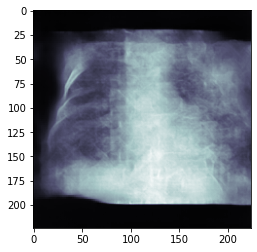
\includegraphics[width=\textwidth]{xray_sample2.png}
         %\caption{MNIST}
     \end{subfigure}
     \hfill
     \begin{subfigure}[b]{0.3\textwidth}
         \centering
         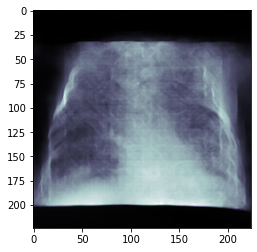
\includegraphics[width=\textwidth]{xray_sample3.png}
         %\caption{FashionMNIST}
     \end{subfigure}
     \hfill
     \begin{subfigure}[b]{0.3\textwidth}
         \centering
         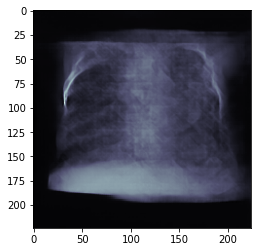
\includegraphics[width=\textwidth]{xray_sample5.png}
         %\caption{MNIST}
     \end{subfigure}
     \hfill
     \begin{subfigure}[b]{0.3\textwidth}
         \centering
         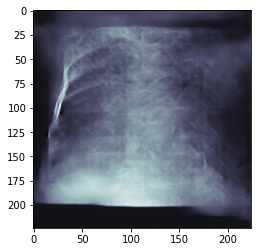
\includegraphics[width=\textwidth]{xray_sample6.png}
         %\caption{FashionMNIST}
     \end{subfigure}
     \caption{Generated x-ray images}
     \label{fig:xray_results}
\end{figure}

Our goal, however, is not to fool a human critic, but our classifier models trained on the data set. So, we generated some images using our model sampled at $\tau = [0.65, 0.7, 0.75, 0.8, 0.85, 0.9]$ (Figure \ref{fig:pneumonia_test_samples}) and put them through our classifiers. We found that both the Alexnet and VGG based classifiers were consistently fooled by the generated images achieving a $96\%$ fooling success rate. However, we obtained a $0\%$ fooling rate for the Resnet-based classifier. 

We believe the high-fooling rate achieved by our generated images is mainly caused by a bias of the Alexnet and VGG classification models towards predicting the Pneumonia class. This bias is probably caused by the fact that the data set is imbalanced toward such class. Nonetheless, the validation set used to report the classifiers performance does not display such a marked imbalance. Thus, we consider our reported classifier performance results to be valid.  

    \begin{figure}[!htbp]
        \centering
        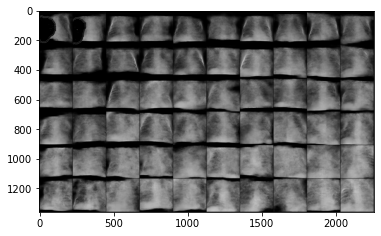
\includegraphics[width=.5\textwidth]{xray_test_example.png}
        \caption{Pneumonia generated images used for testing.}
        \label{fig:pneumonia_test_samples}
    \end{figure}

Finally, we tested our models ability to fool the classifiers to produce the Normal class instead. We trained an equivalent GLOW model with the Normal-labeled images from the dataset ($\sim 3K$) and generated images sampled at $\tau = [0.8, 0.85, 0.9, 0.95]$ (Figure \ref{fig:normal_test_samples}). Using these images we achieved fooling success rates of $65\%$, $32.5\%$, and $42.5\%$ for the Alexnet, VGG, and Resnet classifiers, respectively. Thus confirming our assumptions of our classifiers biases.

    \begin{figure}[!htbp]
        \centering
        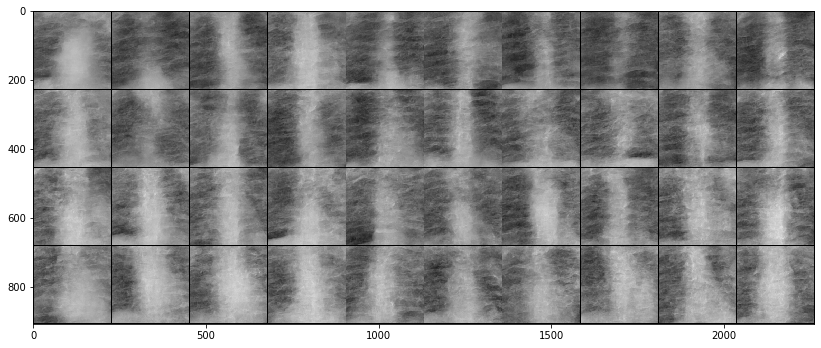
\includegraphics[width=.5\textwidth]{normal_generated.png}
        \caption{Normal generated images used for testing.}
        \label{fig:normal_test_samples}
    \end{figure}



\end{document}
